\subsection{Models}
To implement an API for the WordCount database, we needed communication models for the JSON objects we would be sending to and receiving from the other layers. 
We also needed data access models corresponding to the database relations to access it through EF Core. 
The communication models and the data access models will be described in the following sections.

\subsubsection*{Communication models}
For communication between our layer and the other layers, we have made three input models and one response model. 
These models correspond to the JSON objects we expect to send or receive from other layers when they attempt to insert data into or retrieve data from the database. 
When a JSON object is received, it is parsed into an object from our model, which can then be used to add data to the database.
\\

\textbf{Input models}\\
% ArticleJsonModel
% TermJsonModel
The first input model is \texttt{ArticleJsonModel} which can be seen in figure \ref{ArticlJsonModel}. An article consists of a title, a publisher, a file path, the number of words in the article and an array containing all the words in the article. 
The words are of type \texttt{TermJsonModel} which is a separate model containing the word itself and a number denoting how many times it occurs in the given article.
This model is used when the database receives a JSON object through our endpoint, which corresponds to the \texttt{ArticleJsonModel}. 
After the JSON object has been converted to \texttt{ArticleJsonModel}, the data from the article can be inserted into the WordCount database using EF Core.

\begin{figure}[H]
    \centering
    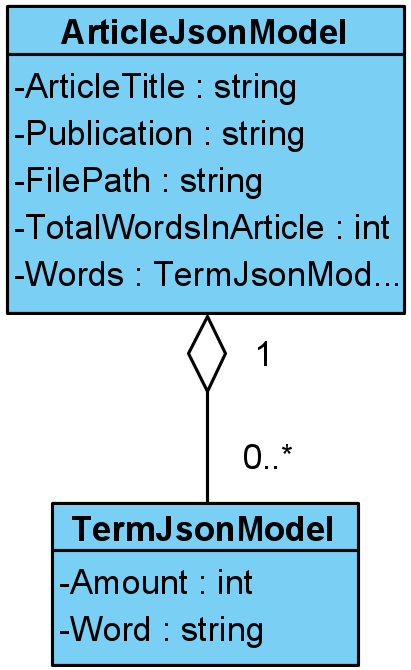
\includegraphics[scale=0.5]{Images/jsonArticleModel.PNG}
    \caption{Diagram of the \texttt{ArticlJsonModel} and the \texttt{TermJsonModel}.}
    \label{ArticlJsonModel}
\end{figure}

% JsonSchemaInputModel
The second input model is \texttt{JsonSchemaInputModel} which can be seen in figure \ref*{JsonSchemaInputModel}. \texttt{JsonSchemaInputModel} contains a name of the JSON schema, and a body which is the JSON schema itself. 
It is used when the other layers try to add JSON schemas to the WordCount database, which is then later used to validate future input. 
How the validation is done will be described in section \ref*{sec:validation}.

\begin{figure}[H]
    \centering
    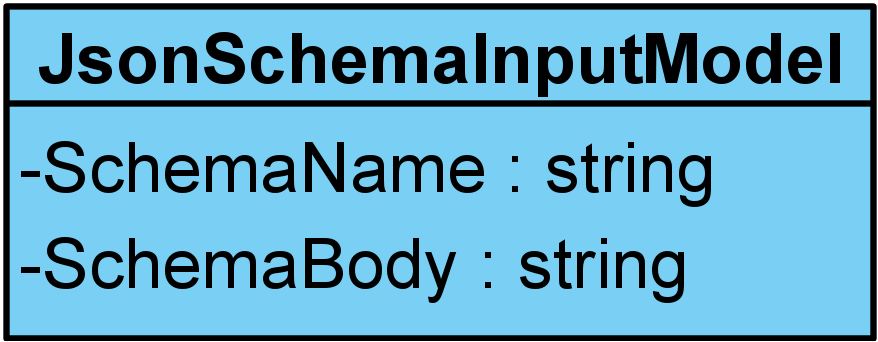
\includegraphics[scale=0.25]{Images/JsonSchemaInputModel.png}
    \caption{Diagram of the \texttt{JsonSchemaInputModel}.}
    \label{JsonSchemaInputModel}
\end{figure}

\textbf{Response Models}\\
% FileIdResponse
The response model \texttt{FileIdResponse} is used when a request for the path of an article is made, and can be seen in figure \ref*{FileIdResponse},
After the path has been queried in the WordCount database, it is put into the response model which is returned as a JSON object.

\begin{figure}[H]
    \centering
    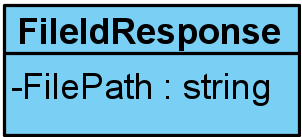
\includegraphics[scale=0.25]{Images/FileIdResponse.png}
    \caption{Diagram of the \texttt{FileIdResponse} model.}
    \label{FileIdResponse}
\end{figure}

\subsubsection*{Data access models}
To use EF Core for data access, we also had to implement models of the relations in the database, which are be used to insert and query data. 
All of these models must be contain exactly the same fields as the relations in the database.
EF Core then maps these models to the relations such that they can be used to manipulate data.
\\
% Article
% publisher
% Term
The model of the \texttt{Article} relation as well as \texttt{Term} and \texttt{Publisher} can be seen in figure \ref*{Article}. 
\begin{figure}[H]
    \centering
    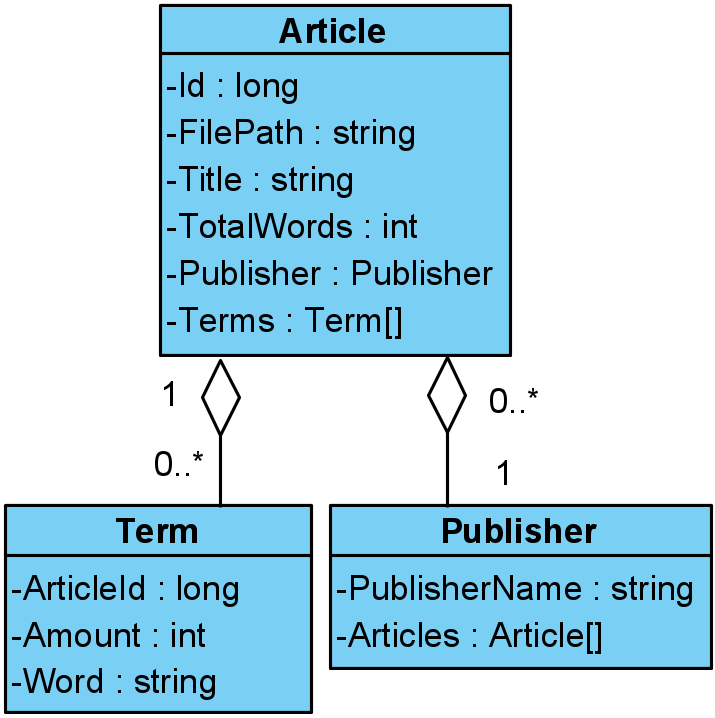
\includegraphics[scale=0.25]{Images/ArticleModel.PNG}
    \caption{Diagram of the Article model}
    \label{Article}
\end{figure}
Similarly, the other models used for database access have been created to replicate the structure of the database. 
The remaining models can be seen in appendix \ref*{AppDataAccess}.